\chapter{MAGIC-UNet results}\label{ch:magic_results}

All MAGIC-UNet runs ran on the server's RTX A6000. Each one generated its own training crops (about 1.7 hours with 24
workers), trained for 50 epochs (about 4 hours, 286 seconds per epoch), then scored itself on simulated images and on every
COMSOL pair. No COMSOL number was used to choose anything.

\section{Run 1: a bug, not a result}

Run 1 trained smoothly, but its scores were terrible: 74\% on simulated images and 82\% on COMSOL at 3\um\ to 0.5\um,
no better than copying the blurry input (75\%). The predicted field was about 3.5 times too small.

The weights were fine. The fault was in BatchNorm. During training, each BatchNorm layer normalises with the statistics of
the current batch, and it also keeps a running average of those statistics to use at test time. We compared the two on
2,048 validation crops:

\begin{center}
\begin{tabular}{lcc}
\toprule
Validation crops, run 1 weights & Current error & Best-fit scale \\
\midrule
Stored running statistics (what was scored) & 93.8\% & 5.8 \\
Statistics of each batch & 17.0\% & 1.00 \\
Running statistics recomputed on clean training batches & 16.8\% & 1.00 \\
\bottomrule
\end{tabular}
\end{center}

The cause was our noise. Run 1 set each layout's noise level from the field range of the \emph{whole} 140\um\ layout.
About 0.5\% of crops lie far from every wire, where the field is tiny. Their noise was therefore huge compared with
their own field, up to 165 times their largest value. Because every crop is divided by its own $\alpha$, those few crops
became enormous noise images, and they corrupted the running variance. Recomputing the statistics with those crops
included gave 98.9\%; without them, 16.8\%.

\begin{figure}[H]
\centering
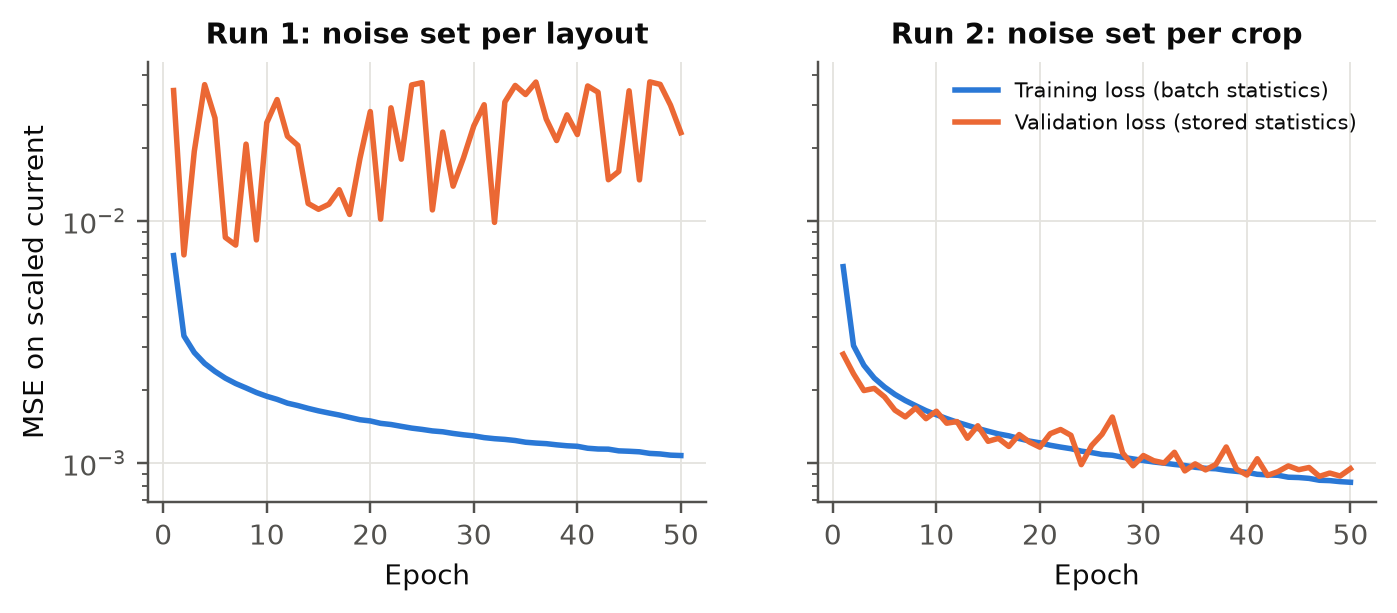
\includegraphics[width=\textwidth]{magic_history}
\caption{Training (blue) and validation (orange) loss. In run 1 the validation loss jumps around and never improves,
because it uses the corrupted stored statistics. In run 2 the two curves follow each other.}
\label{fig:magic_history}
\end{figure}

\begin{careful}[Whose mistake]
This was a flaw in our data design, not in the paper. The paper sets the noise relative to each image's own largest
field. We had copied our simulator's habit of setting it per layout.
\end{careful}

\section{Run 2: the fix}

Run 2 sets the noise from each crop's own field range, as the paper does:

\begin{code*}{magic_data.py}
def crop_sigma(b, percent):
    """White-noise sigma (uT) of one crop b [3, H, W]: percent of its own mean component range."""
    return percent / 100 * float(np.mean(b.max((1, 2)) - b.min((1, 2))))
\end{code*}

The stored crops had no noise in them yet, so they were kept, and a new \code{--resigma} option rewrote only the noise
levels. Run 1 had not saved each crop's percentage, so it was drawn again from the same 1, 1.5, 2 and 2.5\%. Over 20,000
training crops the noise is now at most 4.2\% of a crop's largest field, with a median of 1.4\%.

\begin{careful}
Run 2 is not a pure rerun. Its typical noise is lower than run 1's (1.4\% against 3.0\% of a crop's field), because noise
is no longer inflated far from the wires. Noise level is a setting we chose.
\end{careful}

\subsection{Simulated images}

On 50 full simulated validation images the field error at 0.5\um\ is 15.2\%. The predicted current scores SSIM 0.81 and
0.89 for $J_x$ and $J_y$. Tile stride 32 was chosen here. This number is not comparable with the 48.8\% of
Chapter~\ref{ch:results}, which was scored on 64 signal-rich crops.

\subsection{COMSOL at 3\um\ to 0.5\um}

The score is the same as for every other method: relative $L_2$ per component over the full image, averaged over the same
15 pairs. We checked both scoring paths in the code.

\begin{center}
\small
\begin{tabular}{lcccccccc}
\toprule
Method & Standoff given? & L1\_C1 & IC\_4um & C1+C2 & C1--C3 & C1--C4 & Mean \\
\midrule
\textbf{MAGIC-UNet, run 2} & \textbf{No} & \textbf{26.3\%} & 29.6\% & \textbf{26.6\%} & \textbf{26.4\%} & \textbf{26.0\%} &
\textbf{27.0\%} \\
FISTA-300, $\lambda=0.009$ & Yes & 31.2\% & \textbf{27.6\%} & 31.4\% & 31.2\% & 31.1\% & 30.5\% \\
FISTA-Net, run 2 & Yes & 33.1\% & 34.6\% & 33.2\% & 33.1\% & 32.7\% & 33.3\% \\
\bottomrule
\end{tabular}
\end{center}

\begin{figure}[H]
\centering
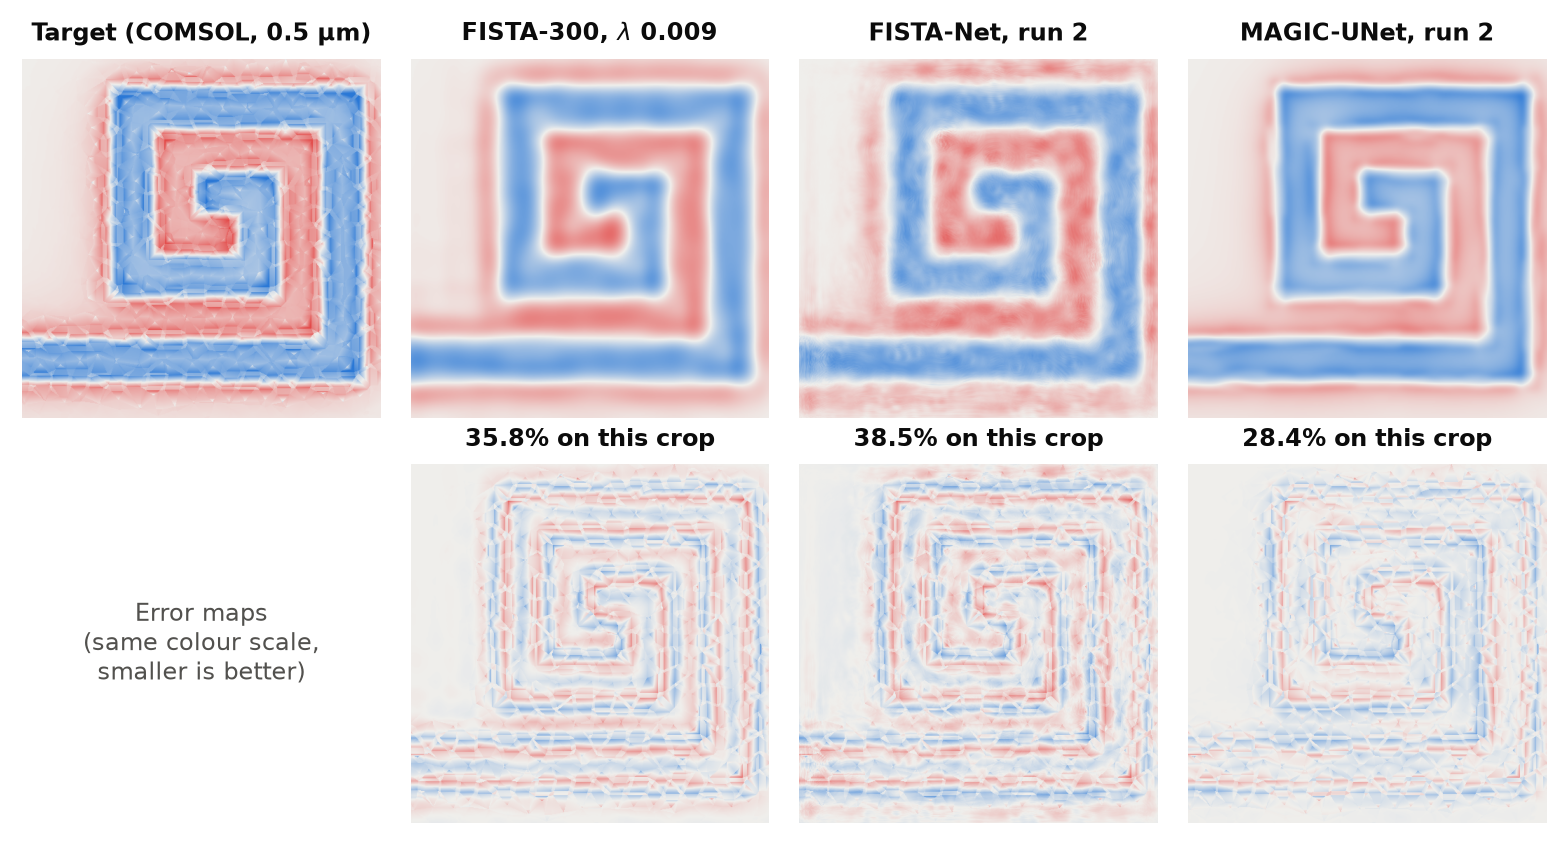
\includegraphics[width=\textwidth]{magic_reconstruction}
\caption{$B_z$ of L1\_C1 at 0.5\um, the same $512\times512$ crop as Chapter~\ref{ch:results}. MAGIC-UNet ran on the full
image and was then cropped; FISTA-300 and FISTA-Net ran on the crop alone, so MAGIC-UNet had more surrounding context.}
\label{fig:magic_reconstruction}
\end{figure}

The maps show the difference: the wire edges are cleaner, and the error maps are fainter along the wires. No tile seams
are visible.

\subsection{Other standoffs}

The same network, never told the height, was scored on every other COMSOL pair. Trained heights were 1.2 to 4.8\um.

\begin{center}
\small
\begin{tabular}{lcccccccccc}
\toprule
Input height (\textmu m), target 0.5\um & 1 & 2 & 3 & 4 & 5 & 6 & 7 & 8 & 9 & 10 \\
\midrule
Mean error & 59\% & 32\% & 27\% & 37\% & 52\% & 67\% & 78\% & 87\% & 92\% & 94\% \\
Inside the trained range & no & yes & yes & yes & no & no & no & no & no & no \\
\bottomrule
\end{tabular}
\end{center}

IC\_2um at 2\um\ to 1\um\ scores 26.6\%. Most heights have one or two coils, so only the 3\um\ column is a 15-pair score.

\begin{figure}[H]
\centering
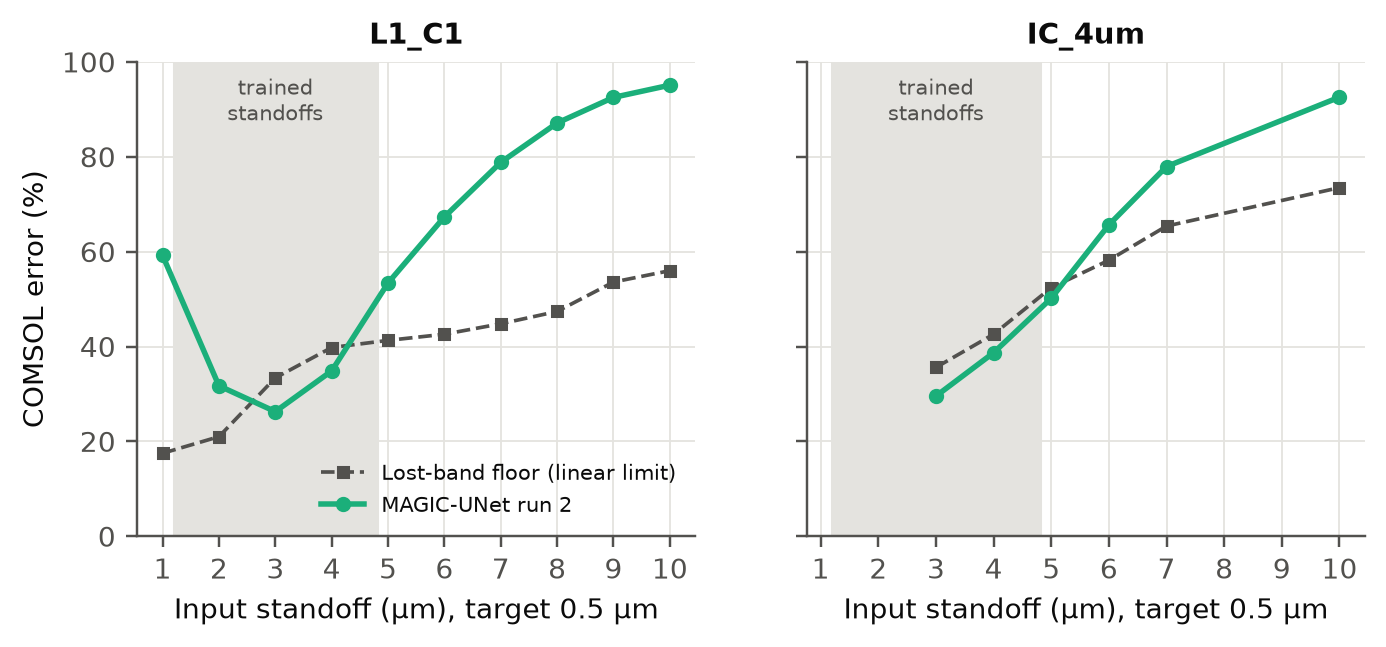
\includegraphics[width=\textwidth]{magic_standoff}
\caption{MAGIC-UNet error against input standoff for each coil, with the lost-band floor of Chapter~\ref{ch:floor}. The
grey band is the range of standoffs seen in training.}
\label{fig:magic_standoff}
\end{figure}

\begin{keyidea}[What run 2 shows]
\begin{itemize}
\item \textbf{Inside the trained range, one network handles an unknown standoff.} At 3\um\ it beats every method that was
given the height. At 3 and 4\um\ on both coils it even goes below the lost-band floor, so its learned prior fills in part
of the lost band. At 2\um\ it stays above the floor.
\item \textbf{Outside the range it fails quickly,} in both directions. At 1\um\ it is far worse than the floor, even though
that input is less blurred than anything it trained on. The network learned to expect a certain amount of blur.
\end{itemize}
\end{keyidea}

\section{Run 3: any standoff}

You asked whether one network could cover every standoff. The architecture needs no change, because the network never sees
the height. Only the training range changes. To keep the comparison explainable, run 3 changes \textbf{exactly one thing}
from run 2:

\begin{center}
\begin{tabular}{lcc}
\toprule
 & Run 2 & Run 3 \\
\midrule
Training standoff & $3\pm0.6$\um, 1.2--4.8\um & uniform over 1--10\um \\
Everything else & \multicolumn{2}{c}{identical: network, $64\times64$ tiles, crops, noise, recipe, scoring} \\
\bottomrule
\end{tabular}
\end{center}

The range 1--10\um\ is exactly the span of the COMSOL inputs. The paper trained one model per standoff range, so a single
1--10\um\ model is our adaptation. Larger tiles were considered for large standoffs and dropped, to stay close to the
paper. Run 3 was launched on 8 November. Its results are in Chapter~\ref{ch:run3}.

\begin{careful}[What to expect from run 3]
At large standoffs most of the target is missing from the data (Chapter~\ref{ch:floor}: 56--73\% at 10\um), so no method will
score well there. The questions are whether 1\um\ and 5--10\um\ improve on run 2, and how much a single any-standoff
network loses at 3\um\ compared with run 2's 27.0\%.
\end{careful}

\section{Is MAGIC-UNet the clear winner?}

Not yet. It is the best result we have, but the claim has limits.
\begin{enumerate}
\item \textbf{Only two geometries.} C2--C4 mirror C1, so the five configurations hold two wire shapes. MAGIC-UNet wins
clearly on the L1/C1 shape (about 26\% against 31\%) and loses on the IC coil (29.6\% against 27.6\%). That is one win and
one loss.
\item \textbf{One training run.} FISTA gives the same answer every time; a trained network does not. Without more seeds we
cannot say how solid a 3.5-point lead is.
\item \textbf{Not like-for-like.} MAGIC-UNet trained on 2,400 layouts and sees all three field components together.
Strict CSC-LISTA and FISTA-Net trained on 200 layouts and see one component at a time. The fair claim is ``MAGIC-UNet, as
we set it up, beats them'', not ``the architecture is better''. Size and data volume alone are unlikely to explain it:
MAGIC-UNet has 15.5 million parameters against 49 million for strict CSC-LISTA at 64 layers (and 75 thousand for
FISTA-Net), and 8,000 layouts made CSC-LISTA worse (Chapter~\ref{ch:followups}).
\item \textbf{No baselines at other standoffs.} Nothing else has been scored at 2 or 4\um\ yet.
\item \textbf{Only what we tried.} Diffusion priors and the untrained network of Dubois et al.\ have not been tested.
\item \textbf{The research question asks for more.} MAGIC-UNet reconstructs well without the height, but it does not
estimate the height or say how sure it is.
\end{enumerate}

\begin{keyidea}[The fair summary]
MAGIC-UNet is the best reconstruction method we have tested at 3\um\ to 0.5\um, and the first that does not need the
standoff. Its lead holds on one of the two coil shapes. It is a strong reconstruction baseline, not yet the complete method
the research question asks for.
\end{keyidea}

\section{What would settle it}

\begin{enumerate}
\item \textbf{FISTA-300 at 2 and 4\um}, once given the true height and once assuming 3\um. This is the baseline for the
unknown-standoff claim, and it takes under an hour.
\item \textbf{Two more seeds of MAGIC-UNet run 2}, about 4 hours each, to see whether 27.0\% holds.
\item \textbf{Run 3's results}, for one network across all standoffs.
\item \textbf{The identifiability check} of Chapter~\ref{ch:question}, before any joint height estimation.
\end{enumerate}

\begin{defend}[If your professor asks: is this just a bigger network winning?]
Not simply. MAGIC-UNet has 15.5 million parameters, fewer than strict CSC-LISTA at 64 layers (49 million), which it beats.
Giving CSC-LISTA forty times more layouts made it worse, so more data alone is not the explanation either. The network is
unmodified from the paper, it never saw COMSOL, and it was not told the standoff, while every method it beats was. It does
see all three components at once, which the others do not, and that may help.
\end{defend}

\begin{defend}[If your professor asks: does it solve the unknown-standoff problem?]
Inside its training range, partly: one network reconstructs at 2, 3 and 4\um\ without being told which. Outside that range
it fails, and it never outputs a height or an uncertainty. Run 3 tests the first point; the second needs the methods in
Chapter~\ref{ch:question}.
\end{defend}

\begin{careful}[Since this chapter was written]
All four steps above were done between 9 and 12 November. They changed the picture: FISTA had been stopped too early,
and the lead of MAGIC-UNet now rests on one added correction step. Read Chapters~\ref{ch:run3} to~\ref{ch:consistency} before
quoting any number from this chapter. Chapter~\ref{ch:ten} takes the method to 10\um.
\end{careful}

\section{What is not yet known}

\begin{itemize}
\item How much MAGIC-UNet's score varies between seeds.
\item Whether its lead holds on a third wire shape. Today it wins on one shape and loses on the other.
\item How FISTA and the other methods do at 2 and 4\um, with and without the true height.
\item Whether one network can cover 1--10\um\ (run 3).
\item Whether any source prior makes the height identifiable on COMSOL.
\item Everything on experimental QDM data. Nothing here has been tested on real measurements.
\end{itemize}
